\section{Decision-Tree Induction}

\begin{frame}{Decision-tree: An Example}
	\begin{columns}
		\begin{column}{0.38\textwidth}
			\vspace{-3cm}
			\begin{itemize}
				\item \textbf{Training dataset: buys\_computer.}
				      \begin{itemize}
					      \item The dataset follows an example of Quinlan's ID3 (playing tennis).
				      \end{itemize}
				\item \textbf{Resulting tree:}\\[0.1cm]
			\end{itemize}
			\centering
			\begin{tikzpicture}
	\node[rounded corners=.25em,draw, fill=faugray!62] at (0,0) (a) {age?};
	\node[rounded corners=.25em,draw] at (-1.5,-0.7) (b) {<=30};
	\node[rounded corners=.25em,draw] at (0,-0.7) (c) {$31\ldots40$};
	\node[rounded corners=.25em,draw] at (1.5,-0.7) (d) {$>40$};
	\node[rounded corners=.25em,draw, fill=faugray!62] at (-1.5,-1.4) (e) {student?};
	\node[rounded corners=.25em,draw] at (-2,-2.1) (eno1) {no};
	\node[rounded corners=.25em,draw] at (-1,-2.1) (eyes1) {yes};
	\node[text=faured] at (-2,-2.8) (eno2) {no};
	\node[text=faugreen] at (-1,-2.8) (eyes2) {yes};
	\node[rounded corners=.25em,draw,fill=faugray!62] at (1.5,-1.4) (g) {credit rating?};
	\node[rounded corners=.25em,draw] at (2.2,-2.1) (gf) {fair};
	\node[rounded corners=.25em,draw] at (1,-2.1) (gex) {excellent};
	\node[text=faured] at (1,-2.8) (gno) {no};
	\node[text=faugreen] at (2.2,-2.8) (gyes) {yes};
	\node[text=faugreen] at (0,-2.8) (f) {yes};

	\draw (a)--(b);
	\draw (a)--(c);
	\draw (a)--(d);
	\draw (b)--(e);
	\draw (c)--(f);
	\draw (d)--(g);
	\draw (e)--(eno1);
	\draw (e)--(eyes1);
	\draw (eno1)--(eno2);
	\draw (eyes1)--(eyes2);
	\draw (g)--(gex);
	\draw (g)--(gf);
	\draw (gex)--(gno);
	\draw (gf)--(gyes);
\end{tikzpicture}

		\end{column}
		\begin{column}{0.62\textwidth}
			\small
			\begin{tabular}{|l|l|c|c|c|}
	\hline
	\rowcolor{faugray!62}\textbf{age} & \textbf{income} & \textbf{student} & \textbf{credit\_rating} & \textbf{buys\_computer} \\\hline
	$\leq 30$                         & high            & no               & fair                    & {\color{faured}no}      \\\hline
	$\leq 30$                         & high            & no               & excellent               & {\color{faured}no}      \\\hline
	$31\ldots40$                      & high            & no               & fair                    & {\color{faugreen}yes}   \\\hline
	$>40$                             & medium          & no               & fair                    & {\color{faugreen}yes}   \\\hline
	$>40$                             & low             & yes              & fair                    & {\color{faugreen}yes}   \\\hline
	$>40$                             & low             & yes              & excellent               & {\color{faured}no}      \\\hline
	$31\ldots40$                      & low             & yes              & excellent               & {\color{faugreen}yes}   \\\hline
	$\leq 30$                         & medium          & no               & fair                    & {\color{faured}no}      \\\hline
	$\leq 30$                         & low             & yes              & fair                    & {\color{faugreen}yes}   \\\hline
	$>40$                             & medium          & yes              & fair                    & {\color{faugreen}yes}   \\\hline
	$\leq 30$                         & medium          & yes              & excellent               & {\color{faugreen}yes}   \\\hline
	$31\ldots40$                      & medium          & no               & excellent               & {\color{faugreen}yes}   \\\hline
	$31\ldots40$                      & high            & yes              & fair                    & {\color{faugreen}yes}   \\\hline
	$>40$                             & medium          & no               & excellent               & {\color{faured}no}      \\\hline
\end{tabular}

		\end{column}
	\end{columns}
\end{frame}


\begin{frame}{Decision-Tree}
	\vspace*{-0.6em}
	\begin{block}{Decision-Tree Induction}
		\textit{Decision-Tree induction} refers to the learning of a decision-tree based on labeled training data.
	\end{block}

	\begin{block}{Decision Tree}
		A \textit{decision tree} is a flowchart-like structure consisting of interconnected internal and leaf nodes.
	\end{block}

	\begin{columns}[t]
		\begin{column}{0.45\textwidth}
			\vspace*{-2em}
			\begin{figure}[t]
				\centering
				\begin{tikzpicture}
	\node[rounded corners=.25em,draw, fill=faugray!62] at (0,0) (a) {age?};
	\node[rounded corners=.25em,draw] at (-1.5,-0.7) (b) {<=30};
	\node[rounded corners=.25em,draw] at (0,-0.7) (c) {$31\ldots40$};
	\node[rounded corners=.25em,draw] at (1.5,-0.7) (d) {$>40$};
	\node[rounded corners=.25em,draw, fill=faugray!62] at (-1.5,-1.4) (e) {student?};
	\node[rounded corners=.25em,draw] at (-2,-2.1) (eno1) {no};
	\node[rounded corners=.25em,draw] at (-1,-2.1) (eyes1) {yes};
	\node[text=faured] at (-2,-2.8) (eno2) {no};
	\node[text=faugreen] at (-1,-2.8) (eyes2) {yes};
	\node[rounded corners=.25em,draw,fill=faugray!62] at (1.5,-1.4) (g) {credit rating?};
	\node[rounded corners=.25em,draw] at (2.2,-2.1) (gf) {fair};
	\node[rounded corners=.25em,draw] at (1,-2.1) (gex) {excellent};
	\node[text=faured] at (1,-2.8) (gno) {no};
	\node[text=faugreen] at (2.2,-2.8) (gyes) {yes};
	\node[text=faugreen] at (0,-2.8) (f) {yes};

	\draw (a)--(b);
	\draw (a)--(c);
	\draw (a)--(d);
	\draw (b)--(e);
	\draw (c)--(f);
	\draw (d)--(g);
	\draw (e)--(eno1);
	\draw (e)--(eyes1);
	\draw (eno1)--(eno2);
	\draw (eyes1)--(eyes2);
	\draw (g)--(gex);
	\draw (g)--(gf);
	\draw (gex)--(gno);
	\draw (gf)--(gyes);
\end{tikzpicture}

			\end{figure}

		\end{column}
		\begin{column}{0.55\textwidth}
			\textbf{Components of a Decision-tree}
			\begin{itemize}
				\item \tikzmark{root} \textbf{Root}: topmost node.
				\item \tikzmark{internal} \textbf{Internal node}: test on an attribute.
				\item \tikzmark{leaf-node} \textbf{Leaf node}: holds a class label, also called \textit{terminal node}.
				\item \tikzmark{branch} \textbf{Branch}: outcome of a leaf node's test coupled with a text. In this example: \texttt{excellent}.
			\end{itemize}
		\end{column}
	\end{columns}

	\begin{tikzpicture}[remember picture,overlay]
		\draw[faucyan,thick,->] ([yshift=1.5mm,xshift=-4mm]root) to[out=170,in=0] (age.east);
		\draw[faucyan,thick,->] ([yshift=1.5mm,xshift=-4mm]internal) to[out=180,in=10] (credit-rating.east);
		\draw[faucyan,thick,->] ([yshift=1.5mm,xshift=-4mm]leaf-node) to[out=190,in=30] (credit-yes.east);
		\draw[faucyan,thick,->] ([xshift=-3mm]branch) to[out=-120,in=-90] ([xshift=1mm]$(credit-no.north east) + (.1em,.7em));
	\end{tikzpicture}
\end{frame}



\begin{frame}{Algorithm for Decision-tree Induction}
	\begin{itemize}
		\item \textbf{Basic algorithm (a greedy algorithm):}
		      \begin{itemize}
			      \item Tree is constructed in a \textbf{\color{airforceblue}top-down recursive divide-and-conquer manner.}
			      \item Attributes are categorical.
			            \begin{itemize}
				            \item If not: discretize in advance.
			            \end{itemize}
			      \item At start, all the training examples are at the root.
			      \item Examples are \textbf{\color{airforceblue}partitioned recursively} based on selected attributes.
			      \item Test attributes are selected on the basis of a heuristic or statistical measure.
			            \begin{itemize}
				            \item E.g., information gain -- see on the next slide.
			            \end{itemize}
		      \end{itemize}
		\item \textbf{Conditions for stopping partitioning:}
		      \begin{itemize}
			      \item All samples for a given node belong to the same class.
			      \item There are no remaining attributes for further partitioning.
			            \begin{itemize}
				            \item Majority voting is employed for classifying the leaf.
			            \end{itemize}
			      \item There are no samples left (i.e. partition for particular value is empty).
		      \end{itemize}
	\end{itemize}
\end{frame}

\begin{frame}{Attribute-selection Measure: Information Gain (ID3/C4.5)}
	\textbf{Select the attribute with the highest information gain.}
	\begin{itemize}
		\item Let $p_i$ be the probability that an arbitrary tuple in $D$ belongs to class $C_i$,\\ estimated by $\frac{|C_i|}{|D|}$, such that $1 \leq i \leq m$.
		\item \textbf{Expected information} (entropy) needed to classify a tuple in $D$:
		      \begin{align}
			      \text{Info}(D) = -\sum_{i=1}^{m}p_i \log_2(p_i).
		      \end{align}
		\item \textbf{Information} needed (after using attribute $A$ to split $D$ into $v$ partitions) to classify $D$:
		      \begin{align}
			      \text{Info}_A(D) = \sum_{j=1}^v \left( \frac{|D_j|}{|D|} \text{Info}(D_j) \right).
		      \end{align}
		\item \textbf{Information gained} by branching on $A$:
		      \begin{align}
			      \text{Gain}(A)=\text{Info}(D)-\text{Info}_A(D).
		      \end{align}
	\end{itemize}
\end{frame}

\begin{frame}{Attribute Selection: Information Gain}
	\begin{columns}
		\begin{column}{0.45\textwidth}
			\begin{itemize}
				\item \textbf{Class P: buys\_computer = "yes"}
				\item \textbf{Class N: buys\_computer = "no"}
				      \begin{align*}
					      \resizebox{7cm}{!}{%
						      $\text{Info}(D) = I(9,5) = - \frac{9}{14}\log_2(\frac{9}{14})-\frac{5}{14} \log_2(\frac{5}{14}) = 0.94$
					      }
				      \end{align*}
			\end{itemize}
			\centering
			\begin{tabular}{|l|l|l|l|}
				\hline
				\cellcolor{faugray!62}age     & \cellcolor{faugray!62}p & \cellcolor{faugray!62}n & \cellcolor{faugray!62}$l(p,n)$ \\\hline
				\cellcolor{white}$\leq 30$    & 2                       & 3                       & 0.971                          \\\hline
				\cellcolor{white}$31\ldots40$ & 4                       & 0                       & 0                              \\\hline
				\cellcolor{white}$>40$        & 3                       & 2                       & 0.971                          \\\hline
			\end{tabular}\\[0.2cm]
			\begin{itemize}
				\item \textbf{Similarly,}
				      \begin{itemize}
					      \item $\text{Gain}(\texttt{income}) = 0.029$,
					      \item $\text{Gain}(\texttt{student}) = 0.090$,
					      \item $\text{Gain}(\texttt{credit\_rating}) = 0.048$.
				      \end{itemize}
			\end{itemize}
		\end{column}
		\begin{column}{0.45\textwidth}
			\vspace{-1.3cm}
			\begin{align*}
				\resizebox{7cm}{!}{%
				$\text{Info}_{\texttt{age}}(D) = \frac{5}{14}I(2,3) + \frac{4}{14} I(4,0) + \frac{5}{14} I(3,2) = 0.694$.
				}
			\end{align*}
			$\frac{5}{14} I(2,3)$ means "$\texttt{age} \leq 30$" has $5$ out of $14$ samples, with $2$ yes'es and $3$ no's. Hence,
			\begin{align*}
				\text{Gain}(\texttt{age}) = \text{Info}(D)-\text{Info}_{\texttt{age}}(D) = 0.246.
			\end{align*}

			\resizebox{6cm}{!}{%
				\centering
				\begin{tabular}{|l|l|c|c|c|}
	\hline
	\rowcolor{faugray!62}\textbf{age} & \textbf{income} & \textbf{student} & \textbf{credit\_rating} & \textbf{buys\_computer} \\\hline
	$\leq 30$                         & high            & no               & fair                    & {\color{faured}no}      \\\hline
	$\leq 30$                         & high            & no               & excellent               & {\color{faured}no}      \\\hline
	$31\ldots40$                      & high            & no               & fair                    & {\color{faugreen}yes}   \\\hline
	$>40$                             & medium          & no               & fair                    & {\color{faugreen}yes}   \\\hline
	$>40$                             & low             & yes              & fair                    & {\color{faugreen}yes}   \\\hline
	$>40$                             & low             & yes              & excellent               & {\color{faured}no}      \\\hline
	$31\ldots40$                      & low             & yes              & excellent               & {\color{faugreen}yes}   \\\hline
	$\leq 30$                         & medium          & no               & fair                    & {\color{faured}no}      \\\hline
	$\leq 30$                         & low             & yes              & fair                    & {\color{faugreen}yes}   \\\hline
	$>40$                             & medium          & yes              & fair                    & {\color{faugreen}yes}   \\\hline
	$\leq 30$                         & medium          & yes              & excellent               & {\color{faugreen}yes}   \\\hline
	$31\ldots40$                      & medium          & no               & excellent               & {\color{faugreen}yes}   \\\hline
	$31\ldots40$                      & high            & yes              & fair                    & {\color{faugreen}yes}   \\\hline
	$>40$                             & medium          & no               & excellent               & {\color{faured}no}      \\\hline
\end{tabular}

			}
		\end{column}
	\end{columns}
\end{frame}

\begin{frame}{Partitioning in the Example}
	\centering
	\begin{tikzpicture}
		\node[rounded corners=0.25em,draw, fill=faugray!62] at (0,0) (r) {age?};
		\node[rounded corners=0.25em,draw] at (-2,-1) (a) {$\leq 30$};
		\node[rounded corners=0.25em,draw] at (0,-1) (b) {$31\ldots40$};
		\node[rounded corners=0.25em,draw] at (2,-1) (c) {$>40$};
		\draw (r)--(a);
		\draw (r)--(b);
		\draw (r)--(c);
		\node at (-4,-3) (t1) {
			\begin{tabular}{|l|l|l|l|}
				\hline
				\cellcolor{faugray!62}income & \cellcolor{faugray!62}student & \cellcolor{faugray!62}credit\_rating & \cellcolor{brown!20}buys\_computer \\\hline
				\cellcolor{white}high        & \cellcolor{white}no           & \cellcolor{white}fair                & {\color{faured}no}                 \\\hline
				\cellcolor{white}high        & \cellcolor{white}no           & \cellcolor{white}excellent           & {\color{faured}no}                 \\\hline
				\cellcolor{white}medium      & \cellcolor{white}no           & \cellcolor{white}fair                & {\color{faured}no}                 \\\hline
				\cellcolor{white}low         & \cellcolor{white}yes          & \cellcolor{white}fair                & {\color{faugreen}yes}              \\\hline
				\cellcolor{white}medium      & \cellcolor{white}yes          & \cellcolor{white}excellent           & {\color{faugreen}yes}              \\\hline
			\end{tabular}
		};
		\node at (-2.5,-5.2) (t3) {
			\begin{tabular}{|l|l|l|l|}
				\hline
				\cellcolor{faugray!62}income & \cellcolor{faugray!62}student & \cellcolor{faugray!62}credit\_rating & \cellcolor{brown!20}buys\_computer \\\hline
				\cellcolor{white}high        & \cellcolor{white}no           & \cellcolor{white}fair                & {\color{faugreen}yes}              \\\hline
				\cellcolor{white}low         & \cellcolor{white}yes          & \cellcolor{white}excellent           & {\color{faugreen}yes}              \\\hline
				\cellcolor{white}medium      & \cellcolor{white}no           & \cellcolor{white}excellent           & {\color{faugreen}yes}              \\\hline
				\cellcolor{white}high        & \cellcolor{white}yes          & \cellcolor{white}fair                & {\color{faugreen}yes}              \\\hline
			\end{tabular}
		};
		\node at (2.8,-3.8) (t2) {
			\begin{tabular}{|l|l|l|l|}
				\hline
				\cellcolor{faugray!62}income & \cellcolor{faugray!62}student & \cellcolor{faugray!62}credit\_rating & \cellcolor{brown!20}buys\_computer \\\hline
				\cellcolor{white}medium      & \cellcolor{white}no           & \cellcolor{white}fair                & {\color{faugreen}yes}              \\\hline
				\cellcolor{white}low         & \cellcolor{white}yes          & \cellcolor{white}fair                & {\color{faugreen}yes}              \\\hline
				\cellcolor{white}low         & \cellcolor{white}yes          & \cellcolor{white}excellent           & {\color{faured}no}                 \\\hline
				\cellcolor{white}medium      & \cellcolor{white}yes          & \cellcolor{white}fair                & {\color{faugreen}yes}              \\\hline
				\cellcolor{white}medium      & \cellcolor{white}no           & \cellcolor{white}excellent           & {\color{faured}no}                 \\\hline
			\end{tabular}
		};
		\draw (a)--(t1);
		\draw (c)--(t2);
		\draw (b)--(t3);
	\end{tikzpicture}
\end{frame}

\begin{frame}{Computing Information Gain for Continuous-valued Attributes}
	\begin{itemize}
		\item \textbf{Let attribute A be a continuous-valued attribute.}
		\item \textbf{Must determine the best split point for A.}
		      \begin{itemize}
			      \item Sort the values of A in increasing order.
			      \item Typically, the midpoint between each pair of adjacent values \\ is considered as a possible split point.
			            \begin{itemize}
				            \item $\frac{a_i+a_{i+1}}{2}$ is the midpoint between the values of $a_i$ and $a_{i+1}$.
			            \end{itemize}
			      \item The point with the minimum expected information requirement for $A$ \\ is selected as the split point for $A$.
		      \end{itemize}
		\item \textbf{Split:}
		      \begin{itemize}
			      \item $D_1$ is the set of tuples in $D$ satisfying $A \leq$ split point,\\
			            and $D_2$ is the set of tuples in $D$ satisfying $A >$ split point.
		      \end{itemize}
		\item \textbf{So to say: Discretization as you go along.}
		      \begin{itemize}
			      \item For this particular purpose.
		      \end{itemize}
	\end{itemize}
\end{frame}

\begin{frame}{Gain Ratio for Attribute Selection (C4.5)}
	\begin{itemize}
		\item \textbf{Information-gain measure is biased towards attributes with a large number of values.}
		\item \textbf{C4.5 (a successor of ID3) uses gain ratio to overcome the problem (normalization to information gain):}
		      \begin{align}
			      \text{SplitInfo}_A(D) = - \sum_{j=1}^{v} \frac{|D_j|}{|D|} \log_2\left( \frac{|D_j|}{|D|} \right), \\
			      \text{GainRatio}(A) = \frac{\text{Gain}(A)}{\text{SplitInfo}_A(D)}.
		      \end{align}
		\item Example:
		      \begin{align}
			      \text{SplitInfo}_{\texttt{income}}(D) & = -\frac{4}{14} \log_2 \left( \frac{4}{14} \right) - \frac{6}{14} \log_2 \left( \frac{6}{14} \right) - \frac{4}{14} \log_2 \left( \frac{4}{14} \right) = 1.557, \\
			      \text{GainRatio}(\texttt{income})     & = \frac{0.029}{1.557} = 0.019.
		      \end{align}
		\item The attribute with the maximum gain ratio is selected as the splitting attribute.
	\end{itemize}
\end{frame}

\begin{frame}{Gini Index}
	\begin{itemize}
		\item \textbf{Corrado Gini (1884 -- 1965).}
		      \begin{itemize}
			      \item Italian statistician and sociologist.
		      \end{itemize}
		\item \textbf{Also called Gini coefficient.}
		\item \textbf{Measures statistical dispersion.}
		      \begin{itemize}
			      \item Zero expresses perfect equality where all values belong to the same class.
			      \item One expresses maximal inequality among values.
		      \end{itemize}
		\item \textbf{Based on the Lorenz curve.}
		      \begin{itemize}
			      \item Plots the proportion of the total sum of values ($y$-axis) that is cumulatively assigned to the bottom $x\%$ of the population.
			      \item Line at $45$ degrees thus represents perfect equality of value distribution.
		      \end{itemize}
		\item \textbf{Gini coefficient then is $\ldots$}
		      \begin{itemize}
			      \item $\ldots$ the ratio of the area that lies between the line of equality and the Lorenz curve over the total area under the line of equality.
		      \end{itemize}
	\end{itemize}
\end{frame}

\begin{frame}{Gini Index (II)} % TODO: plot anpassen, sodass cumulative income nur steigt und nie faellt
	\centering
	Example: Distribution of incomes.\\[0.5cm]
	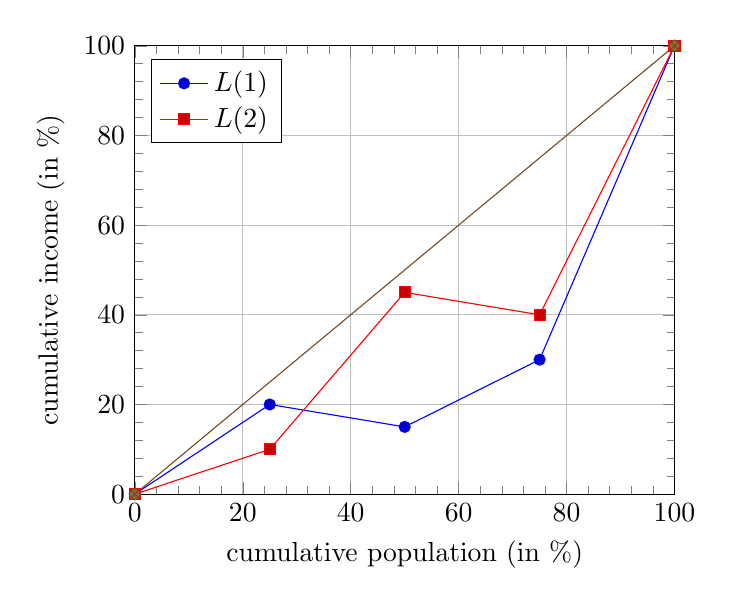
\begin{tikzpicture}
		\begin{axis}[
				xmin=0, xmax=100,
				ymin=0, ymax=100,
				minor tick num = 4,
				grid,
				ylabel = cumulative income (in \%),
				xlabel = cumulative population (in \%),
				legend style={legend pos=north west},
			]
			\addplot plot
			coordinates {(0,0) (25,20) (50,15) (75,30) (100,100)};
			\addplot plot
			coordinates {(0,0) (25,10) (50,45) (75,40) (100,100)};
			\addplot plot [thin]
			coordinates {(0,0) (100,100)};
			\legend{$L(1)$,$L(2)$}
		\end{axis}
	\end{tikzpicture}
\end{frame}

\begin{frame}{Gini Index (CART, IBM IntelligentMiner)}
	\begin{itemize}
		\item \textbf{If a dataset D contains examples from n classes, Gini index gini(D) is defined as:}
		      \begin{align}
			      \text{gini}(D) = 1-\sum_{j=1}^{n} p_j^2,
		      \end{align}
		      where $p_j$ is the relative frequency of class $j$ in $D$.
		\item \textbf{If a dataset $D$ is split on $A$ into two subsets $D_1$ and $D_2$, the Gini index $\text{gini}(D)$ is defined as}
		      \begin{align}
			      \text{gini}_A(D) = \frac{|D_1|}{|D|}\text{gini}(D_1)+\frac{|D_2|}{|D|}\text{gini}(D_2).
		      \end{align}
		\item \textbf{Reduction in impurity:}
		      \begin{align}
			      \Delta \text{gini}_A(D) = \text{gini}(D)-\text{gini}_A(D).
		      \end{align}
		\item \textbf{The attribute $A$ provides the smallest $\text{gini}_A(D)$ (or the largest reduction in impurity) \\ is chosen to split the node.}
		      \begin{itemize}
			      \item Need to enumerate all the possible splitting points for each attribute.
		      \end{itemize}
	\end{itemize}
\end{frame}


\begin{frame}{Computation of Gini Index (I)}
	\begin{itemize}
		\item \textbf{Example:}
		      \begin{itemize}
			      \item $D$ has $9$ tuples in $\text{buys\_computer} =$ "yes" and 5 in "no", thus
			            \begin{align}
				            \text{gini}(D) = 1 - \left( \frac{9}{14} \right)^2 - \left( \frac{5}{14} \right)^2 = 0.459.
			            \end{align}
		      \end{itemize}
		\item Suppose the attribute $\texttt{income}$ partitions $D$ \\ into $10$ in $D_1:\{\texttt{low,medium}\}$ and $4$ in $D_2: \{\texttt{high}\}$:
		      \begin{align}
			       & \text{gini}(D\vert_{D[\texttt{income}]="medium", "low"})                                                                                                                                   \\
			       & = \frac{10}{14} \text{gini}(D_1) + \frac{4}{14} \text{gini}(D_2)                                                                                                                           \\
			       & =\frac{10}{14} \left(1-\left( \frac{7}{10} \right)^2 - \left( \frac{3}{10} \right)^2 \right) + \frac{4}{14} \left( 1-\left( \frac{2}{4} \right)^2 - \left( \frac{2}{4} \right)^2 \right) = \\
			       & = 0.443 = \text{gini}(D\vert_{D[\texttt{income}]="high"}).
		      \end{align}
	\end{itemize}
\end{frame}

\begin{frame}{Computation of Gini Index (II)}
	\begin{itemize}
		\item \textbf{Example (cont.):}
		      \begin{itemize}
			      \item $\text{gini}(D\vert_{D[\texttt{income}]="low", "high"}) = 0.458$,\\
			            $\text{gini}(D\vert_{D[\texttt{income}]="medium", "high"}) = 0.450.$
			      \item Thus, split on the \{"low","medium"\} and \{"high"\}, since it has the lowest gini index.
		      \end{itemize}
		\item \textbf{All attributes are assumed continuous-valued.}
		\item \textbf{May need other tools, E.g., clustering, to get the possible split values.}
		\item \textbf{Can be modified for categorical attributes.}
	\end{itemize}
\end{frame}

\begin{frame}{Computation of Gini Index (III)}
	\begin{itemize}
		\item \textbf{The three measures, in general, return good results, but}
		      \begin{itemize}
			      \item \textbf{\color{airforceblue}Information gain:}
			            \begin{itemize}
				            \item Biased towards multi-valued attributes.
			            \end{itemize}
			      \item \textbf{\color{airforceblue}Gain ratio:}
			            \begin{itemize}
				            \item Tends to prefer unbalanced splits in which one partition is much smaller than the others.
			            \end{itemize}
			      \item \textbf{\color{airforceblue}Gini index:}
			            \begin{itemize}
				            \item Biased to multi-valued attributes.
				            \item Has difficulty when number of classes is large.
				            \item Tends to favor tests that result in equal-sized partitions and purity in both partitions.
			            \end{itemize}
		      \end{itemize}
	\end{itemize}
\end{frame}

\begin{frame}{Other Attribute-selection Measures}
	\begin{itemize}
		\item \textbf{CHAID:}
		      \begin{itemize}
			      \item A popular decision-tree algorithm, measure based on $\chi^2$ test for independence.
		      \end{itemize}
		\item \textbf{C-SEP:}
		      \begin{itemize}
			      \item Performs better than information gain and Gini index in certain cases.
		      \end{itemize}
		\item \textbf{G-statistic:}
		      \begin{itemize}
			      \item Has a close approximation to $\chi^2$ distribution.
		      \end{itemize}
		\item \textbf{MDL (Minimal Description Length) principle:}
		      \begin{itemize}
			      \item I.e. the simplest solution is preferred.
			      \item The best tree is the one that requires the fewest number of bits to both (1) encode the tree and (2) encode the exceptions to the tree.
		      \end{itemize}
		\item \textbf{Multivariate splits:}
		      \begin{itemize}
			      \item Partitioning based on multiple variable combinations.
			      \item CART: finds multivariate splits based on a linear combination of attributes.
		      \end{itemize}
		\item \textbf{Which attribute-selection measure is the best?}
		      \begin{itemize}
			      \item Most give good results, none is significantly superior to others.
		      \end{itemize}
	\end{itemize}
\end{frame}

\begin{frame}{Overfitting and Tree Pruning}
	\begin{itemize}
		\item \textbf{Overfitting: An induced tree may overfit the training data.}
		      \begin{itemize}
			      \item Too many branches, some may reflect anomalies due to noise or outliers.
			      \item Poor accuracy for unseen samples.
		      \end{itemize}
		\item \textbf{Two approaches to avoid overfitting:}
		      \begin{itemize}
			      \item \textbf{\color{airforceblue}Prepruning:}
			            \begin{itemize}
				            \item Halt tree construction early.\\
				                  Do not split a node, if this would result in the goodness measure falling below a threshold.
				            \item Difficult to choose an appropriate threshold.
			            \end{itemize}
			      \item \textbf{\color{airforceblue}Postpruning:}
			            \begin{itemize}
				            \item Remove branches from a "fully grown" tree.\\
				                  Get a sequence of progressively pruned trees.
				            \item Use a set of data different from the training data to decide which is the "best pruned tree."
			            \end{itemize}
		      \end{itemize}
	\end{itemize}
\end{frame}

\begin{frame}{Enhancements to Basic Decision-Tree Induction}
	\begin{itemize}
		\item \textbf{Allow for} \textbf{\color{airforceblue}continuous-valued attributes.}
		      \begin{itemize}
			      \item Dynamically define new discrete-valued attributes that partition the values of continuous-valued attributes into a discrete set of intervals.
		      \end{itemize}
		\item \textbf{Handle} \textbf{\color{airforceblue}missing attribute values.}
		      \begin{itemize}
			      \item Assign the most common value of the attribute.
			      \item Assign probability to each of the possible values.
		      \end{itemize}
		\item \textbf{\color{airforceblue}Attribute construction.}
		      \begin{itemize}
			      \item Create new attributes based on existing ones that are sparsely represented.
			      \item This reduces fragmentation, repetition, and replication.
		      \end{itemize}
	\end{itemize}
\end{frame}

\begin{frame}{Classification in Large Databases}
	\begin{itemize}
		\item \textbf{Classification -- a classical problem extensively \\ studied by statisticians and machine-learning researchers.}
		\item \textbf{Scalability:}
		      \begin{itemize}
			      \item Classifying datasets with millions of examples and \\ hundreds of attributes with reasonable speed.
		      \end{itemize}
		\item \textbf{Why is decision-tree induction popular?}
		      \begin{itemize}
			      \item Relatively fast learning speed (compared to other classification methods).
			      \item Convertible to simple and easy-to-understand classification rules.
			      \item Can use SQL queries for accessing databases.
			      \item Classification accuracy comparable with other methods.
		      \end{itemize}
		\item \textbf{RainForest (Gehrke, Ramakrishnan \& Ganti, VLDB'98).}
		      \begin{itemize}
			      \item Builds an AVC-list (attribute, value, class\_label).
		      \end{itemize}
	\end{itemize}
\end{frame}

\begin{frame}{Scalability Framework for RainForest}
	\begin{itemize}
		\item \textbf{Separates the scalability aspects from the criteria that determine the quality of the tree.}
		\item \textbf{Builds an} \textbf{\color{airforceblue}AVC-list:}.
		      \begin{itemize}
			      \item AVC (Attribute, Value, Class\_label).
		      \end{itemize}
		\item \textbf{\color{airforceblue}AVC-set} \textbf{(of an attribute X):}
		      \begin{itemize}
			      \item Projection of training dataset onto the attribute $X$ and class label where counts of individual class label are aggregated.
		      \end{itemize}
		\item \textbf{\color{airforceblue}AVC-group} \textbf{(of a node n):}
		      \begin{itemize}
			      \item Set of AVC-sets of all predictor attributes at the node $n$.
		      \end{itemize}
	\end{itemize}
\end{frame}

\begin{frame}{RainForest: Training Set and its AVC-sets}
	\begin{columns}
		\begin{column}{0.6\textwidth}
			\small
			\begin{tabular}{|l|l|c|c|c|}
	\hline
	\rowcolor{faugray!62}\textbf{age} & \textbf{income} & \textbf{student} & \textbf{credit\_rating} & \textbf{buys\_computer} \\\hline
	$\leq 30$                         & high            & no               & fair                    & {\color{faured}no}      \\\hline
	$\leq 30$                         & high            & no               & excellent               & {\color{faured}no}      \\\hline
	$31\ldots40$                      & high            & no               & fair                    & {\color{faugreen}yes}   \\\hline
	$>40$                             & medium          & no               & fair                    & {\color{faugreen}yes}   \\\hline
	$>40$                             & low             & yes              & fair                    & {\color{faugreen}yes}   \\\hline
	$>40$                             & low             & yes              & excellent               & {\color{faured}no}      \\\hline
	$31\ldots40$                      & low             & yes              & excellent               & {\color{faugreen}yes}   \\\hline
	$\leq 30$                         & medium          & no               & fair                    & {\color{faured}no}      \\\hline
	$\leq 30$                         & low             & yes              & fair                    & {\color{faugreen}yes}   \\\hline
	$>40$                             & medium          & yes              & fair                    & {\color{faugreen}yes}   \\\hline
	$\leq 30$                         & medium          & yes              & excellent               & {\color{faugreen}yes}   \\\hline
	$31\ldots40$                      & medium          & no               & excellent               & {\color{faugreen}yes}   \\\hline
	$31\ldots40$                      & high            & yes              & fair                    & {\color{faugreen}yes}   \\\hline
	$>40$                             & medium          & no               & excellent               & {\color{faured}no}      \\\hline
\end{tabular}

		\end{column}
		\begin{column}{0.3\textwidth}
			\vspace{-3cm}

			\centering
			AVC-set on age:\\
			\begin{tabular}{|c|c|c|}
				\hline
				age          & yes & no \\\hline
				$\leq 30$    & 2   & 3  \\\hline
				$31\ldots40$ & 4   & 0  \\\hline
				$>40$        & 3   & 2  \\\hline
			\end{tabular}\\[1cm]
			AVC-set on income:\\
			\begin{tabular}{|c|c|c|}
				\hline
				income & yes & no \\\hline
				high   & 2   & 2  \\\hline
				medium & 4   & 2  \\\hline
				low    & 3   & 1  \\\hline
			\end{tabular}
		\end{column}
	\end{columns}
\end{frame}

\begin{frame}{RainForest: Training Set and its AVC-sets (II)}
	\begin{columns}
		\begin{column}{0.6\textwidth}
			\small
			\begin{tabular}{|l|l|c|c|c|}
	\hline
	\rowcolor{faugray!62}\textbf{age} & \textbf{income} & \textbf{student} & \textbf{credit\_rating} & \textbf{buys\_computer} \\\hline
	$\leq 30$                         & high            & no               & fair                    & {\color{faured}no}      \\\hline
	$\leq 30$                         & high            & no               & excellent               & {\color{faured}no}      \\\hline
	$31\ldots40$                      & high            & no               & fair                    & {\color{faugreen}yes}   \\\hline
	$>40$                             & medium          & no               & fair                    & {\color{faugreen}yes}   \\\hline
	$>40$                             & low             & yes              & fair                    & {\color{faugreen}yes}   \\\hline
	$>40$                             & low             & yes              & excellent               & {\color{faured}no}      \\\hline
	$31\ldots40$                      & low             & yes              & excellent               & {\color{faugreen}yes}   \\\hline
	$\leq 30$                         & medium          & no               & fair                    & {\color{faured}no}      \\\hline
	$\leq 30$                         & low             & yes              & fair                    & {\color{faugreen}yes}   \\\hline
	$>40$                             & medium          & yes              & fair                    & {\color{faugreen}yes}   \\\hline
	$\leq 30$                         & medium          & yes              & excellent               & {\color{faugreen}yes}   \\\hline
	$31\ldots40$                      & medium          & no               & excellent               & {\color{faugreen}yes}   \\\hline
	$31\ldots40$                      & high            & yes              & fair                    & {\color{faugreen}yes}   \\\hline
	$>40$                             & medium          & no               & excellent               & {\color{faured}no}      \\\hline
\end{tabular}

		\end{column}
		\begin{column}{0.3\textwidth}
			\vspace{-3cm}

			\centering
			AVC-set on student:\\
			\begin{tabular}{|c|c|c|}
				\hline
				student & yes & no \\\hline
				yes     & 6   & 1  \\\hline
				no      & 3   & 4  \\\hline
			\end{tabular}\\[1cm]
			AVC-set on credit\_rating:\\
			\begin{tabular}{|c|c|c|}
				\hline
				credit\_rating & yes & no \\\hline
				fair           & 6   & 2  \\\hline
				excellent      & 3   & 3  \\\hline
			\end{tabular}
		\end{column}
	\end{columns}
\end{frame}

\begin{frame}{BOAT (Bootstrapped Optimistic Algorithm for Tree Construction)}
	\begin{itemize}
		\item \textbf{Use a statistical technique called bootstrapping to create several smaller samples (subsets), each fitting in memory.}
		      \begin{itemize}
			      \item See on the subsequent slides.
		      \end{itemize}
		\item \textbf{Each subset is used to create a tree, resulting in several trees.}
		\item \textbf{These trees are examined and used to construct a new tree T'.}
		      \begin{itemize}
			      \item It turns out that T' is very close to the tree that would be generated \\
			            using the whole data set together.
		      \end{itemize}
		\item \textbf{Advantages:}
		      \begin{itemize}
			      \item Requires only two scans of DB.
			      \item An incremental algorithm:
			            \begin{itemize}
				            \item Take insertions and deletions of training data and update the decision tree.
			            \end{itemize}
		      \end{itemize}
	\end{itemize}
\end{frame}

\begin{frame}{Presentation of Classification Results}
	\centering
	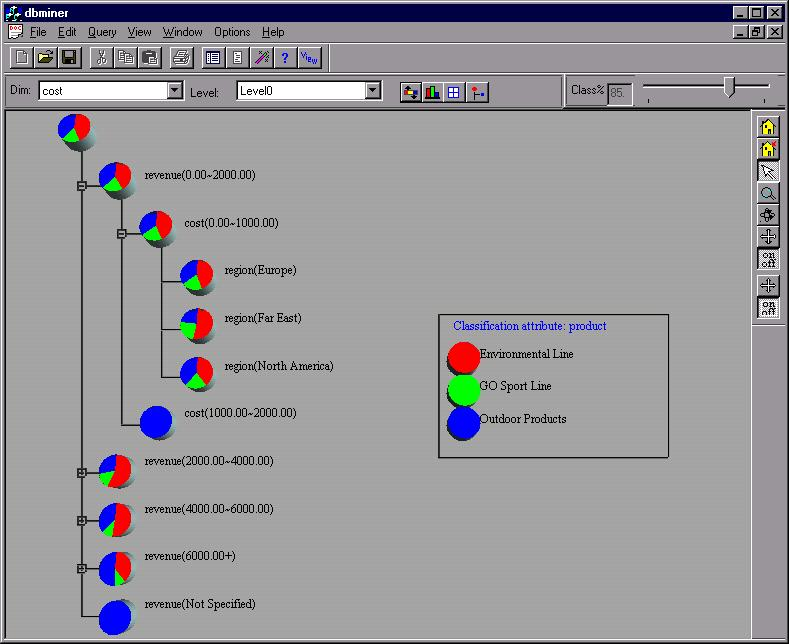
\includegraphics[height=0.8\textheight]{img/classification1.jpeg}
\end{frame}

\begin{frame}{Visualization of a Decision Tree in SGI/MineSet 3.0}
	\centering
	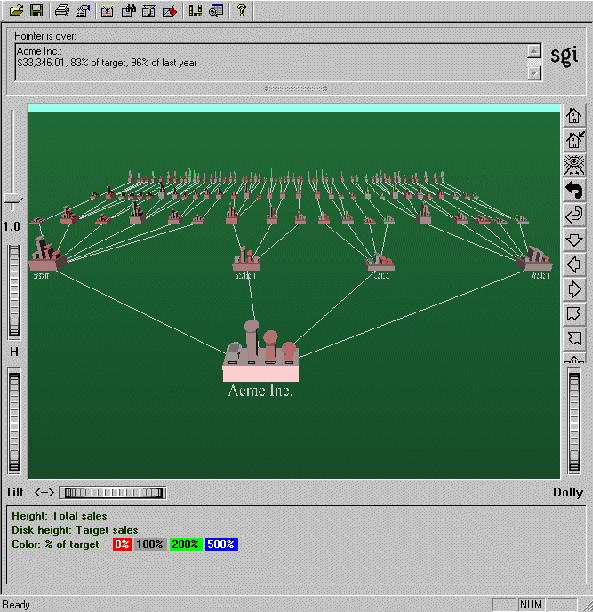
\includegraphics[height=0.8\textheight]{img/classification2.jpeg}
\end{frame}

\begin{frame}{Interactive Visual Mining by Perception-based Classification (PBC)}
	\centering
	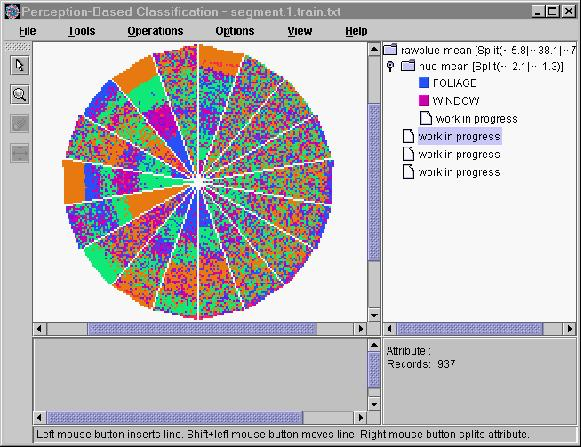
\includegraphics[height=0.8\textheight]{img/classification3.jpeg}
\end{frame}
